\chapter*{Appendix} \label{chp:appendix}
\section*{Proofs}

\begin{proof} \label{proof:insertionSearch}
Given a set of cognitive operations $M$, an external activation function $f()$, an initially valid CTM $\pi=\{s_i \longmapsto m_0\in M \longmapsto ... \longmapsto m_n\in M\}$, and a valid SCP $\mu=(\pi,f)$, inserting multiple operations into $\pi$ to create the CTM $\pi''$ may result in a valid SCP $\mu''=(\pi'',f())$, when inserting only one operation to create $\mu'=(\pi',f())$ would result in an invalid SCP.

\begin{enumerate}
\item Assume hybrid validity (Section~\ref{ssec:precond}).
\item Let $\pi=(s_i)$.
\item Let $s_i$ be of structure $(S,V)$
\item Let $f(\pi)=\top$.
\item Let $\gamma = \top$.
\item Let $\mu=(\pi,f())$ be a valid SCP.
\item Let $m_1 \in M$ be a cognitive operation with output structure $(S)$. And precondition structure $\chi=\{\}$.
\item Let $m_2 \in M$ be a cognitive operation with output structure $(S,V)$. And precondition structure $\chi=\{\}$.
\item Then $\mu'=(\pi',f()), \pi'=(s_i \longmapsto m_1)$ is not a valid SCP.
\item However, $\mu''=(\pi'',f()), \pi''=(s_i \longmapsto m_1 \longmapsto m_2)$ is a valid SCP.
\end{enumerate}
\end{proof}








\begin{proof} \label{proof:infiniteSCPs}
There are an infinite number of possible, valid SCPs, that can meet any goal condition $\gamma$ from input $x$ provided that at least one SCP exists that can reach a final state dependent goal condition $\gamma$ from input $s_i$.
\begin{enumerate}
\item There exists an infinite set  $M^\text{add} \in \Omega$ of unique cognitive operations which add a new variable from the set of all possible variable names $p \in \Sigma$.
\item There exists an infinite set $M^\text{rem} \in \Omega$ of unique cognitive operations  which remove a variable from the set of all possible variable names  $p \in \Sigma$.
\item It follows that there exist infinite set of pairs $M^\text{addRem}$ many pairs $(m^\text{add}_i \in M^\text{add}, m^\text{rem}_i \in M^\text{rem}) \in W$ where $m^\text{add}_i$ adds a variable $p \in \Sigma$ to the resulting state point, and $m^\text{rem}_i$ removes that variable from the resulting statepoint.
\item Then $f(x \longmapsto A) = f(s_i \longmapsto m^\text{add}_i \longmapsto m^\text{rem}_i \longmapsto A)$ for all $(m^\text{add}_i, m^\text{rem}_i) \in M^\text{addRem}$.
\end{enumerate}
\end{proof}






















\begin{proof} \label{proof:infiniteSCPLength}
If there exists an SCP which meets a goal condition $\gamma$ of length $n$, using a final state dependant external evaluation function $f()$ then there exists an SCP that meets $\gamma$ of length $n+k$ where $k$ is any natural number.
\begin{itemize}

\item Proof~\ref{proof:infiniteSCPs} states that if $f(x \longmapsto A)\models \gamma$ then $f(s_i \longmapsto m^\text{add}_i \longmapsto m^\text{rem}_i \longmapsto A)$ for all $(m^\text{add}_i, m^\text{rem}_i) \in M^\text{addRem}$.
\item Let $X$ be a pCTM of the form $X=(m^\text{add}_0 \longmapsto m^\text{rem}_0 \longmapsto ... \longmapsto m^\text{add}_N \longmapsto m^\text{rem}_{N})$ where $(m^\text{add}_i, m^\text{rem}_i) \in M^\text{addRem}$.
\item For odd lengths:
\begin{itemize}
\item  It follows that if $f(x \longmapsto A)\models \gamma$ then $f(x \longmapsto A \longmapsto \textrm{exp}(X))\models \gamma$, where $\textrm{exp}$ denotes the substitution of $X$ for its constituent parts.
\item Because $X$ always contains an even number of cognitive operations, the length of the resulting SCP must be $n' = 1+v$ where $v$ is any even number.
\end{itemize}
\item For even lengths:
\begin{itemize}
\item Let $T \in \Omega$ be the trivial operation, that is, it returns the input state point as output.
\item Notice that $f(x \longmapsto A \longmapsto T) \models \gamma$ iff $f(x \longmapsto A) \models \gamma$.
\item Thus, $f(x \longmapsto A \longmapsto \textrm{exp}(X) \longmapsto T )\models \gamma$ and is of length $n' = 2+v$, where $v$ is any even number.
\end{itemize}
\end{itemize}

\end{proof}

\begin{comment}

\end{comment}
@TODOFIX!!!!
\begin{lemma} \label{lem:uniredundant}
Given a cognitive operation sequence $A \in \Omega^*$, a final state dependant external evaluation function $f()$, and goal $\gamma$, $A$ is redundant iff one of the following holds:
\begin{itemize}
\item $f(x \longmapsto B \longmapsto C) \models x'$ and $f(x \longmapsto A) \models x'$ for every viable epistemic state $x$, $B \in \Omega^*$, $C \in \Omega^*$. 
\item $f(x \longmapsto A) \models x$ for every viable epistemic state $x$.
\item $f(x \longmapsto B)=c$ for all $B \in \Omega^*$, where $c$ is a constant external decision.
\end{itemize}
\end{lemma}



@TODOFIX!!!!
\begin{lemma} \label{lem:taskredundant}
Given a limited set of cognitive operations $M=\{A_0, ..., A_n\}, A_x \in \Omega^*$, a final state dependant external evaluation function  $f()$, and goal $\gamma$, $A \in M^*$ is task redundant iff one of the following holds:
\begin{itemize}
\item $f(x \longmapsto B \longmapsto C) \models \gamma'$ and $f(x \longmapsto A) \models x''$ for every viable epistemic state $x$, $B \in M^*$, $C \in M^*$. 
\item $f(x \longmapsto A) \models x$ for every viable epistemic state $x$.
\item $f(x \longmapsto B)=c$ for all $B \in M^*$, where $c$ is a constant external decision.
\item There exists no epistemic state $x$ and sequences $B, C \in M^*$ such that $f(x \longmapsto B \longmapsto A \longmapsto C)$ is a valid SCP.
\end{itemize}
\end{lemma}




\begin{proof} \label{proof:aggregateExpressiveness}
Given a cognitive task $\Pi=(s_i,f(), M, \gamma)$ in which $M=\{A_0,...,A_n\}$ and a second cognitive planing task $\Pi'=(s_i,f(),M')$ in which $M'= M \smallsetminus \{A_k,...,A_m\} \cup A'$, where $A'=(A_k \longmapsto... \longmapsto A_m)$ is a cognitive sequence containing some ordering of the other operations in $(\Pi \smallsetminus \Pi')$, $\Pi'$ is as expressive or less expressive than $\Pi$.

\item No more expressive:
\begin{itemize}
\item If $\pi' = (s_i\longmapsto A_p \longmapsto ... \longmapsto A' \longmapsto ... \longmapsto A_q)$ and $f(\pi)$ is a solution to $\Pi'$.
\item Let $\pi'' = (s_i\longmapsto A_p \longmapsto ... \longmapsto [A'] \longmapsto ... \longmapsto A_q)$.
\item Then $\mu''=(\pi'',f())$ is a solution to $\Pi'$ (Lemma~\ref{lemma:substitutionValid}).
\item $\mu''$ is a valid solution to $\Pi$ because $\pi''$ uses only cognitive operations which occur in $\Pi$, $s_i$ is the initial epistemic state, and $f(\pi'') \models \gamma$. 
\end{itemize}
\item Less Expressive: Proof by counterexample
\begin{itemize}
\item If we assume that $\Pi'$ is strictly as expressive or more expressive than $\Pi$, then there exist no cases in which $\Pi'$ is less expressive.
\item Let $\gamma = \emptyset$, and $f(x)=True$ for all inputs (i.e. is trivially satisfied).
\item Let $x=\{\}$, $M=\{A_0,A_1\}$, $M'=\{A'\}$, $A'=\{A_0\longmapsto A_1\}$.
\item Then solutions of $\Pi$ are $f(x)$, $f(x \longmapsto A_0)$, $f(x \longmapsto A_1)$, $f(x \longmapsto A_0\longmapsto A_1)$ and $f(x \longmapsto A_1\longmapsto A_0)$.
\item Solutions of $\Pi'$ are $f(x), f(x \longmapsto A')$.
\item Thus, $\Pi'$ has fewer solutions that $\Pi$. A contradiction.
\end{itemize}
\end{proof}

\begin{proof} \label{proof:aggregateValid}
Given an SCP $\mu=(\pi,f())$, $\pi= (s_i \longmapsto A_0 \longmapsto ... \longmapsto A_n)$, where $f()$ is an final state dependant external evaluation function, $s_i$ is a state point, and $A_i \in \Omega$, any subsequence $A'=(A_k \longmapsto ... \longmapsto A_{k+l})$, $(k+l)<n$ of the cognitive operations in $\pi$ is a valid pCTM and, thus, a valid aggregate cognitive operation.
\begin{itemize}
\item Given that $\mu$ is a valid SCP, $s_i \longmapsto A_0$ must result in a valid state point.
\item It follows that $A'$ takes a valid state point as input, because $A_k$ took a valid state point as input.
\item It follows that $A'$ produces a valid state point as output, because $A_{k+1}$ produced a valid state point as output.
\item Therefore, $A'$ is a valid cognitive operation.
\end{itemize}
\end{proof}

\begin{lemma} \label{lemma:substitutionValid}
Let $\pi=(s_i\longmapsto A_0, ..., A', ..., \longmapsto A_n)$ be a CTM drawn from some cognitive task $\Pi=(s_i, \gamma, f(x), M)$ . And let $\pi'=(x\longmapsto [A_0], ..., A', ..., \longmapsto A_n)$ where $[A]$ is the substitution of the aggregate operation $A'$ for $(A'[0]\longmapsto ... \longmapsto A'[t])$ . Then $f(\pi)=f(\pi')$.
\end{lemma}



\section*{Output}
\begin{figure}
\centering 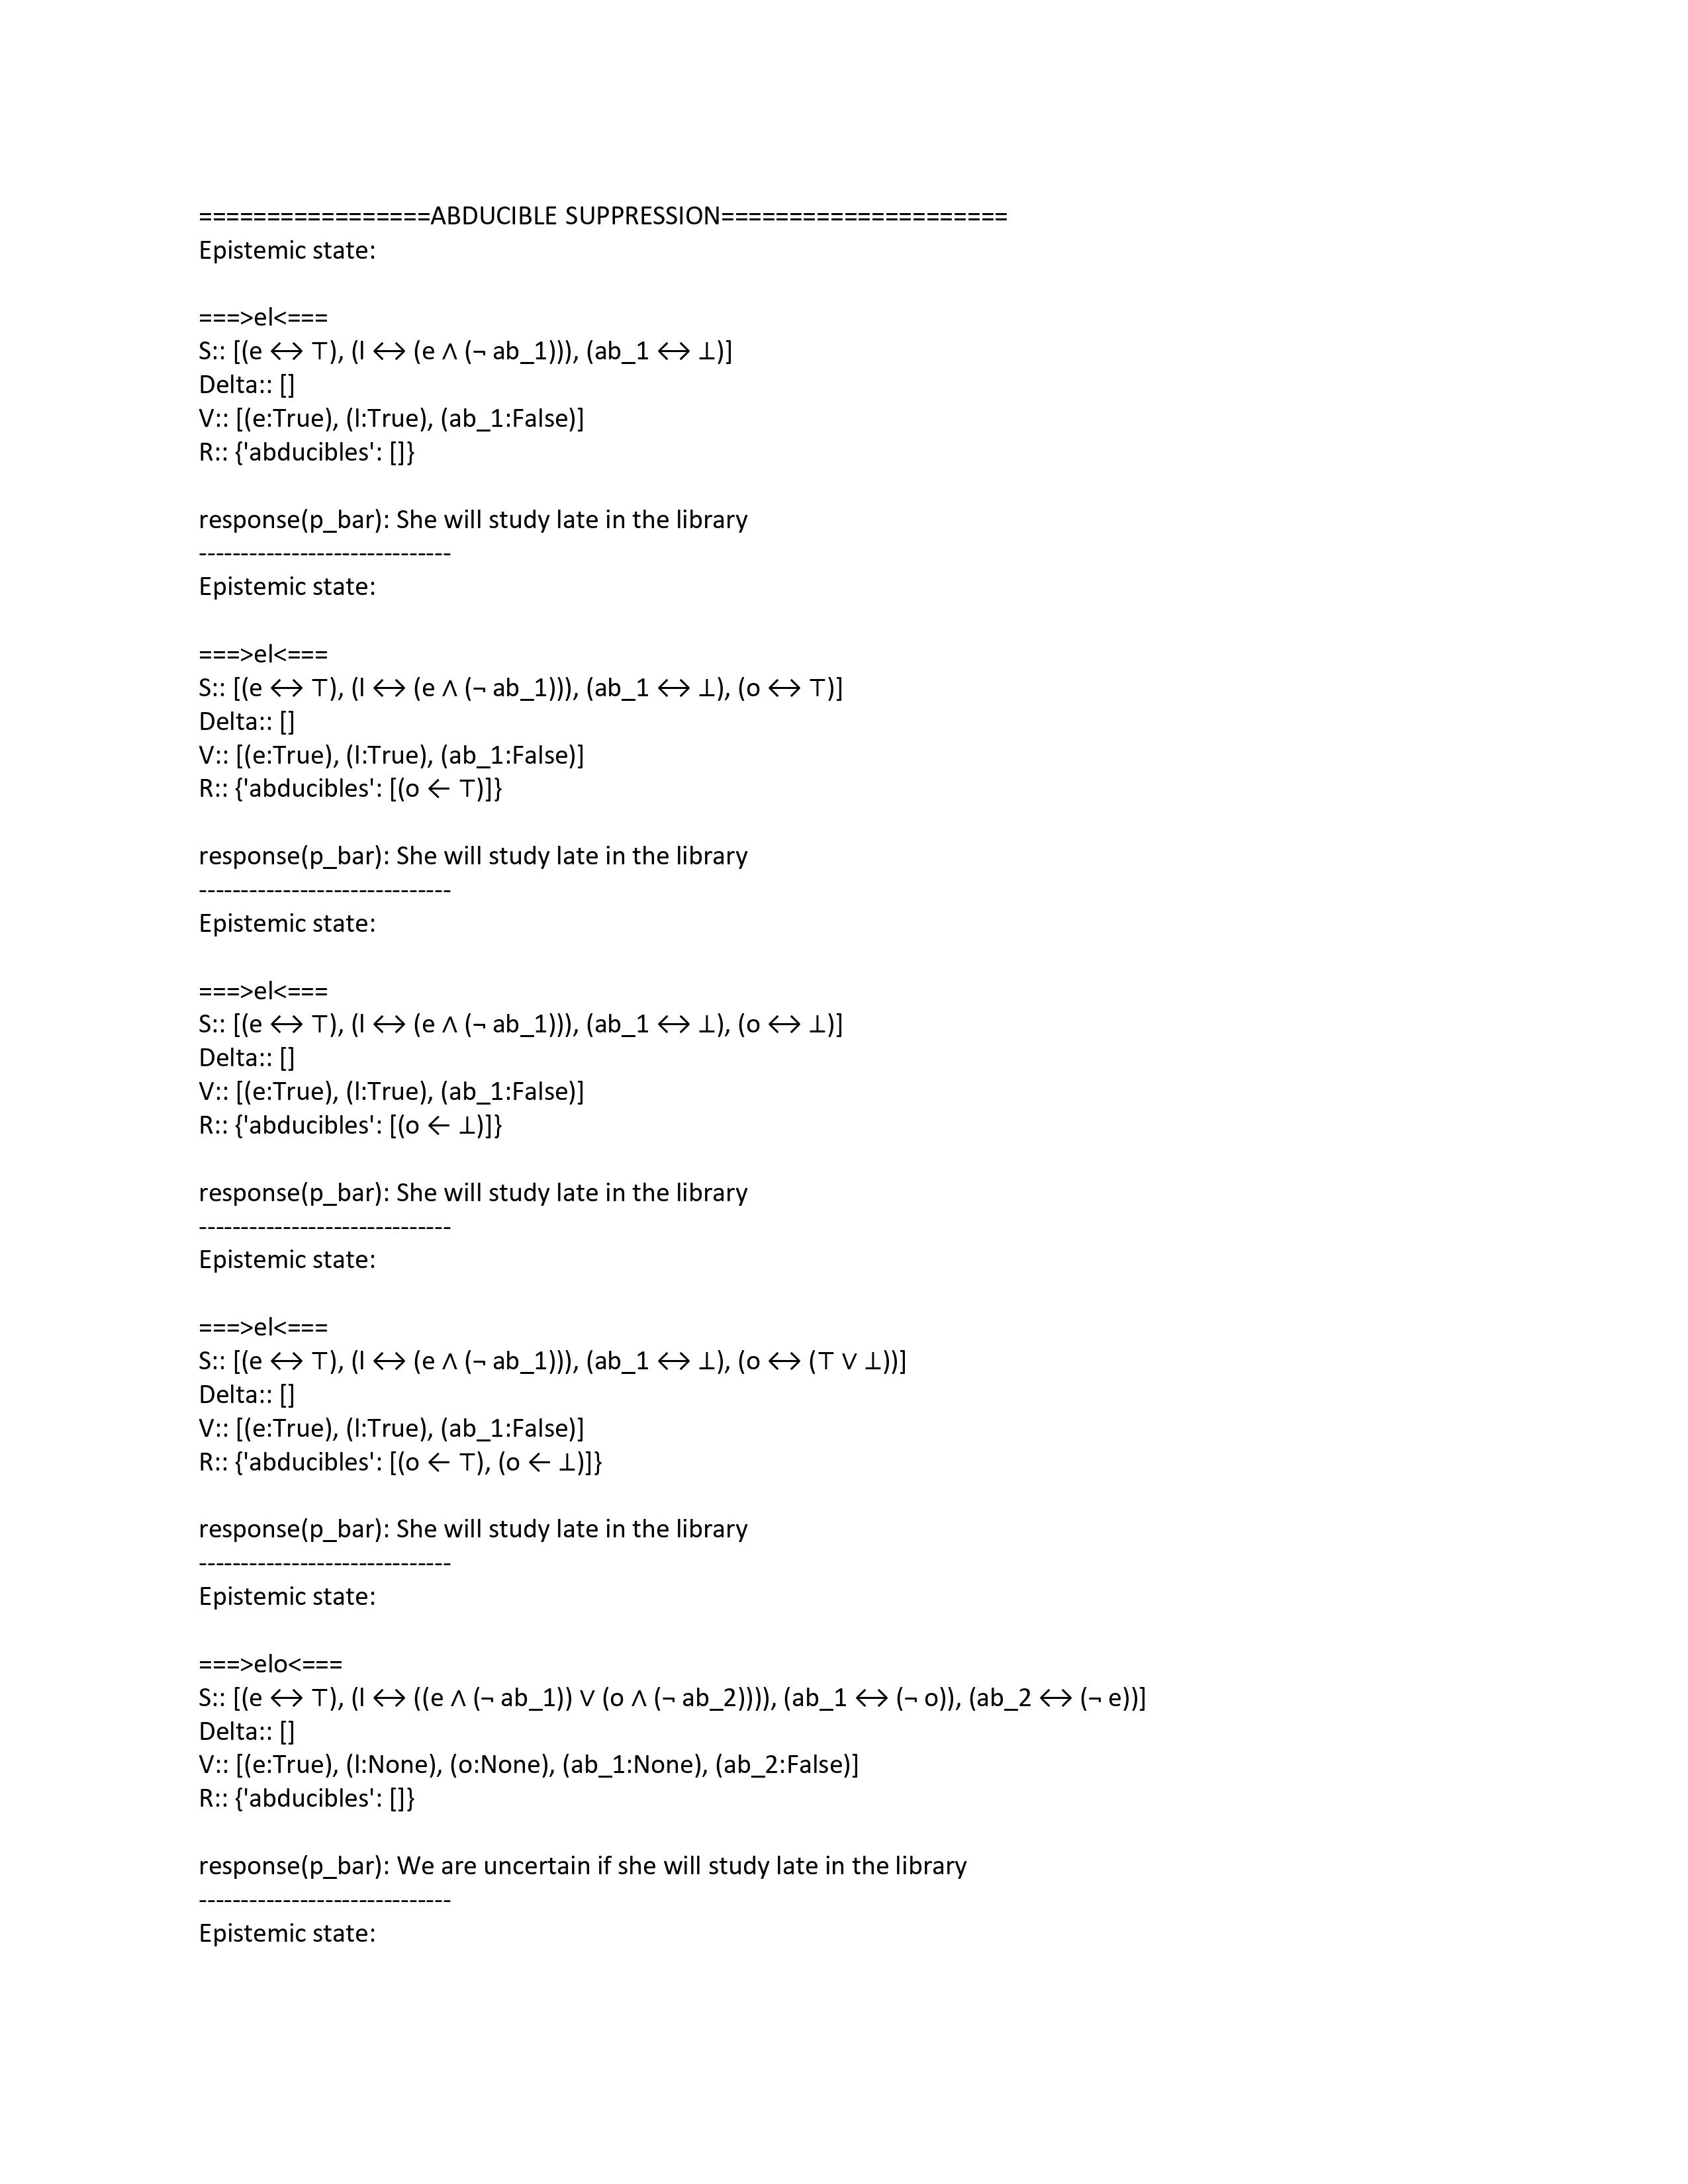
\includegraphics[width=\linewidth]{output1}
\caption{Epistemic states demonstrating that an \texttt{adEXP} can be used to model the individual case of the Suppression Task where Suppression is prevented. Part1.}
\label{fig:suppression_python}
\end{figure}
\begin{figure}
\centering 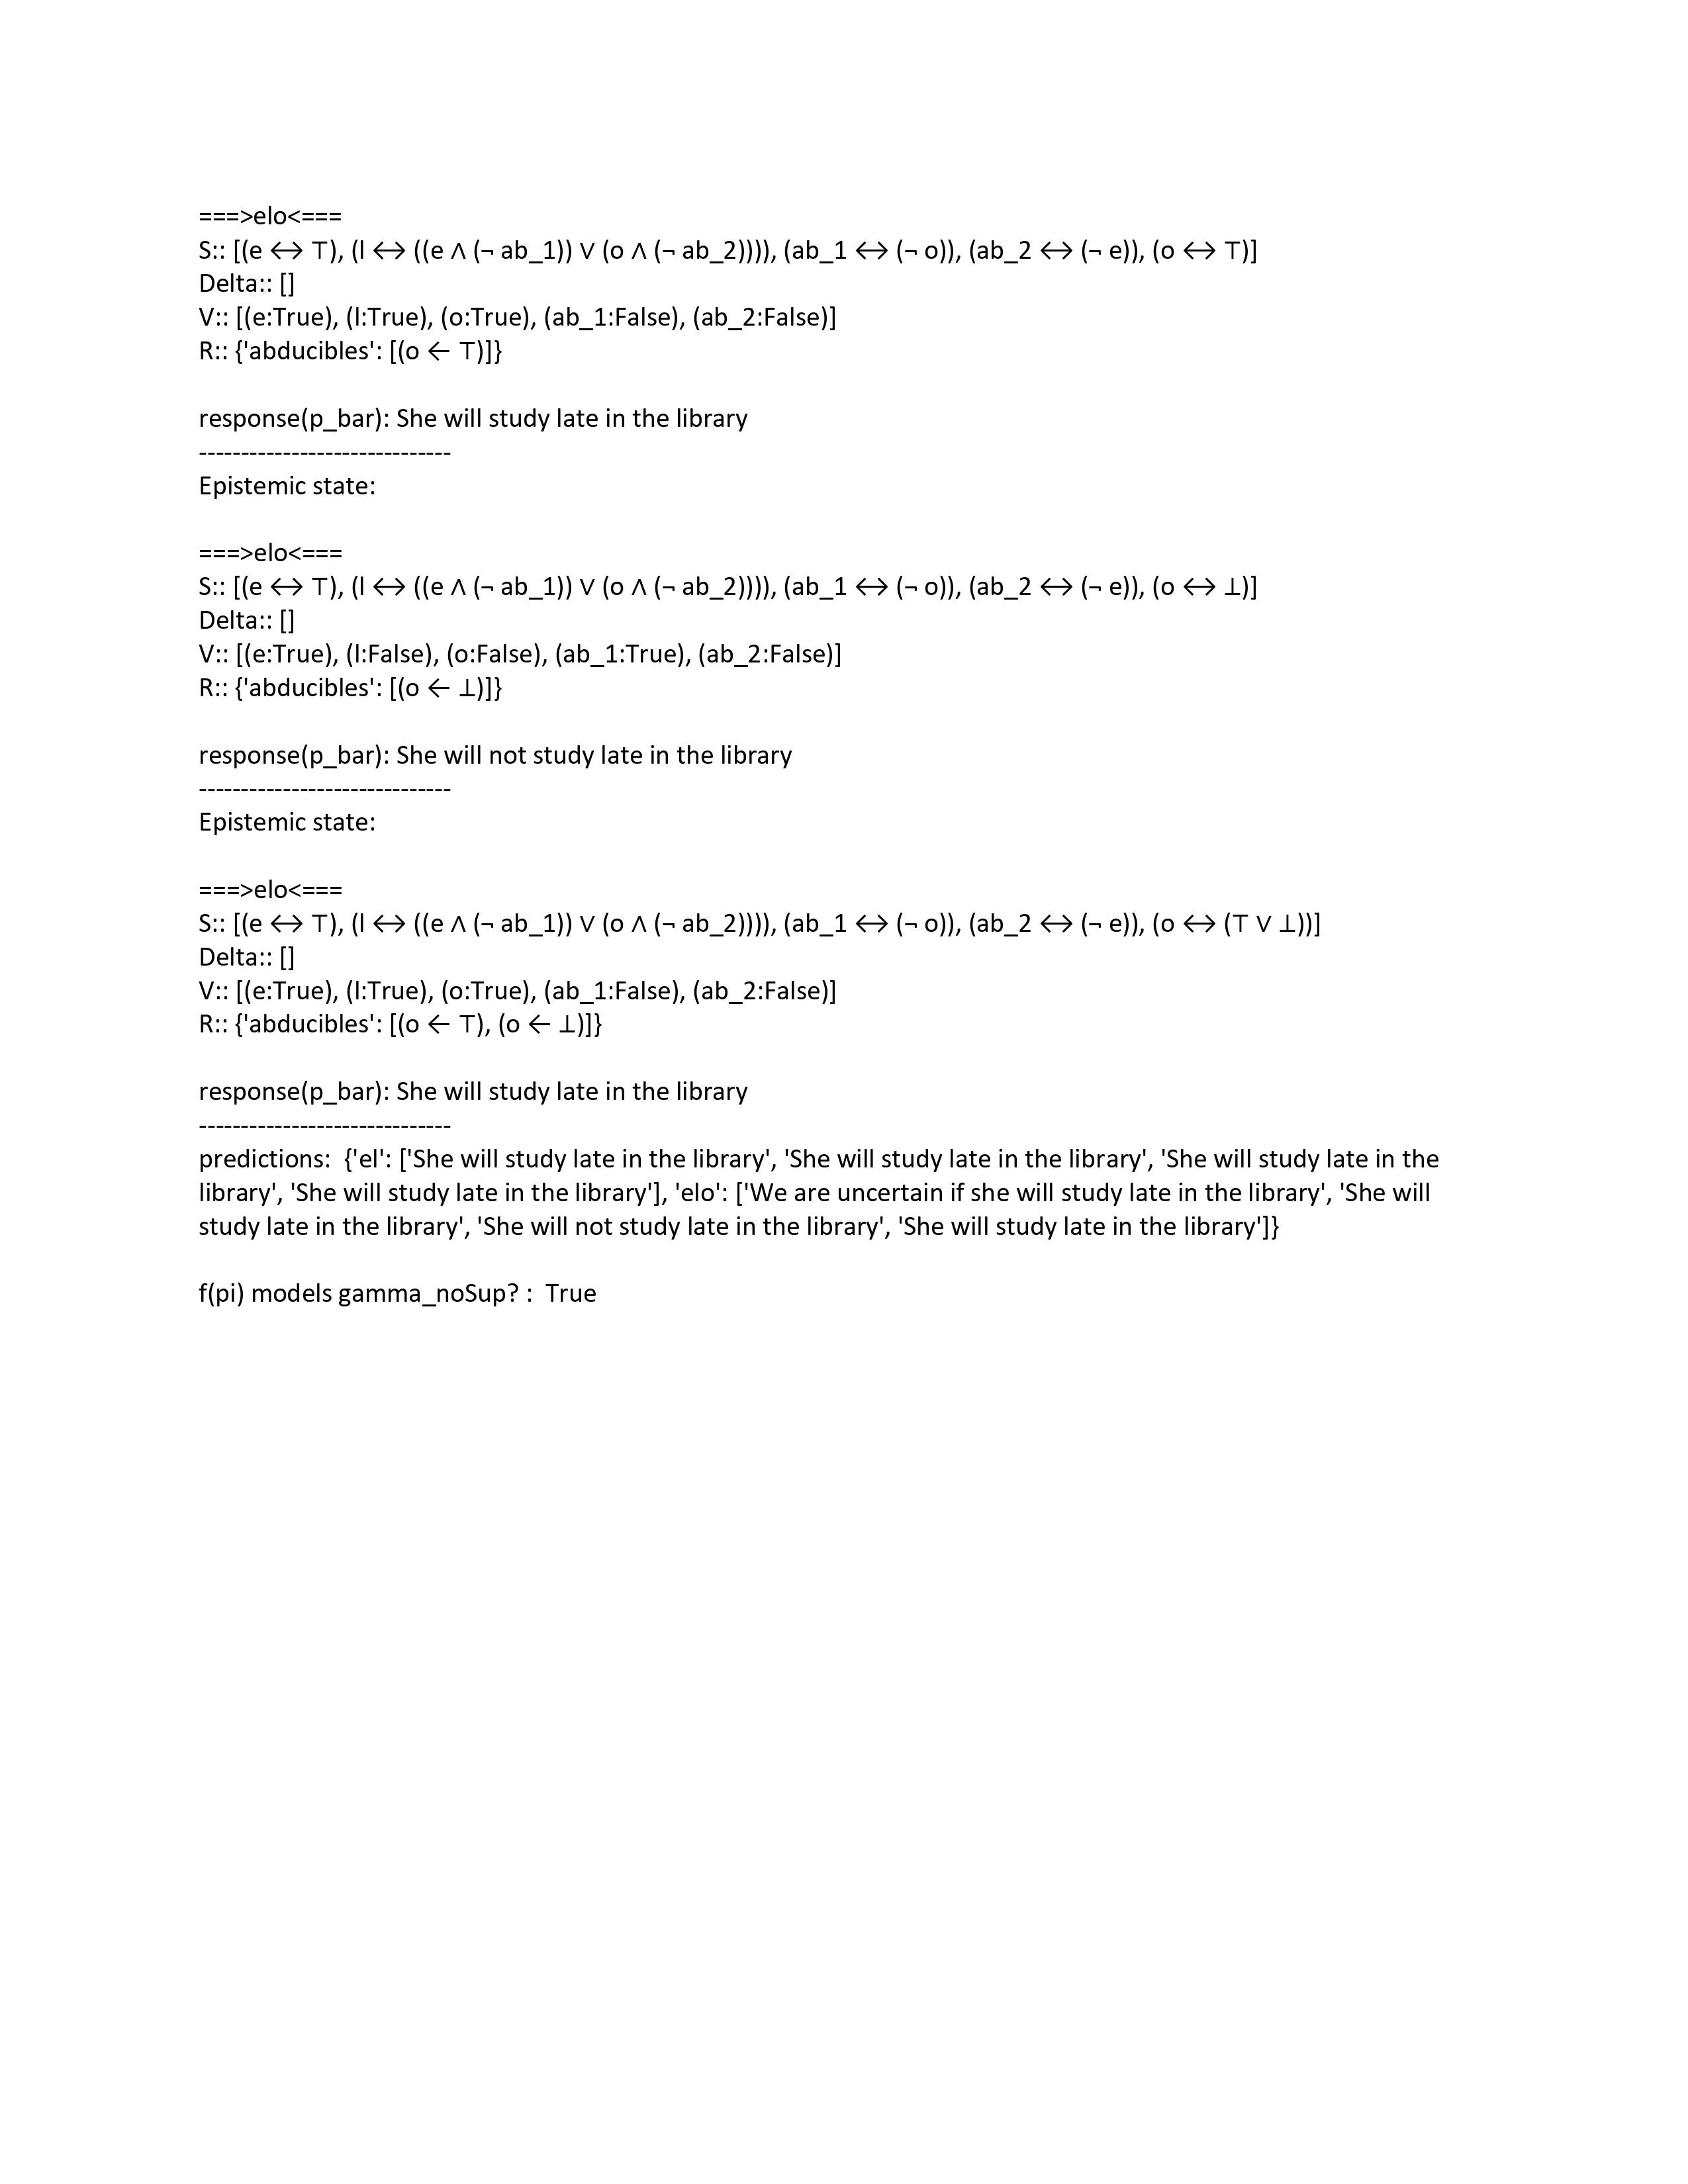
\includegraphics[width=\linewidth]{output2}
\caption{Epistemic states demonstrating that an \texttt{adEXP} can be used to model the individual case of the Suppression Task where Suppression is prevented. Part2.}
\label{fig:suppression_python2}
\end{figure}

\section*{Code Snippets}
\begin{figure}
\centering 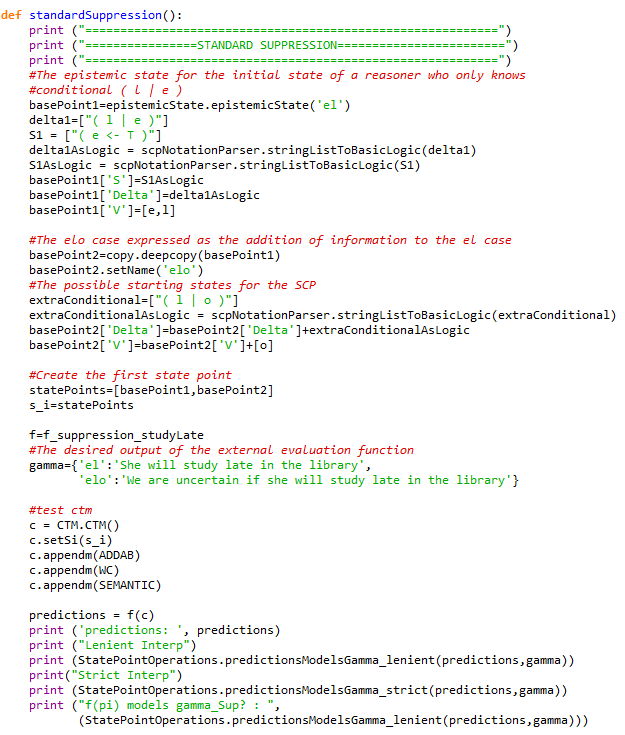
\includegraphics[width=\linewidth]{suppression_python}
\caption{Code snippet showing how the Suppression Task is modelled in the SCP Framework.}
\label{fig:sup_snippet}
\end{figure}

